\documentclass[11pt]{article}
\usepackage[margin=1in]{geometry}
\usepackage{amsmath,amssymb,amsthm}
\usepackage{booktabs,array,tabularx}
\usepackage{graphicx}
\usepackage{enumitem}
\usepackage{float}
\usepackage[hidelinks]{hyperref}
\graphicspath{{figures/}{../figures/}}
\emergencystretch=3em
\setlength{\parindent}{0pt}
\setlength{\parskip}{6pt}
\renewcommand{\arraystretch}{1.2}

% ---------- macros ----------
\newcommand{\R}{\mathbb{R}}
\newcommand{\E}{\mathbb{E}}
\renewcommand{\Pr}{\mathbb{P}}
\newcommand{\tr}{\operatorname{tr}}
\newcommand{\Var}{\operatorname{Var}}
\newcommand{\Cov}{\operatorname{Cov}}
\newcommand{\diag}{\operatorname{diag}}
\newcommand{\one}{\mathbf{1}}
\newcommand{\T}{^{\top}}
\newcommand{\hSigma}{\hat{\Sigma}}
\newcommand{\hmu}{\hat{\mu}}
\newcommand{\norm}[1]{\lVert #1\rVert}

\theoremstyle{plain}
\newtheorem{theorem}{Theorem}
\newtheorem{proposition}{Proposition}
\newtheorem{corollary}{Corollary}
\theoremstyle{definition}
\newtheorem{definition}{Definition}
\theoremstyle{remark}
\newtheorem*{remark}{Remark}

\title{\textbf{Keystroke Anomaly Detection with the Mahalanobis Distance}\\[4pt]
\large DS5020 Final Project, Iteration 2: The Math Foundation}
\author{Nikhil Chaganti \and Trung Pham}
\date{Fall 2026}

\begin{document}
\maketitle
\tableofcontents

% =====================================================================
\section{Overview}
We want to tell whether a password was typed by its owner or by someone else,
using only the timing of the key presses. For one user, we model the timing
vector of each attempt as $x\sim\mathcal N(\mu,\Sigma)$ and estimate $\mu$ and
$\Sigma$ by maximum likelihood from that user's own attempts. A new attempt is
flagged as an anomaly when its squared Mahalanobis distance from $\hmu$ is larger
than the $(1-\alpha)$ quantile of a $\chi^2$ distribution. The real data are the
CMU Keystroke Dynamics Benchmark (Killourhy and Maxion, 2009).

One fact about the data affects the whole method: the 31 timing columns are
exactly linearly dependent, so the $31\times31$ sample covariance has rank 21 and
cannot be inverted (Proposition~\ref{prop:singular}). We therefore drop 10
columns and work with $p=21$ features.

% =====================================================================
\section{Notation}\label{sec:notation}
\begin{table}[H]
\centering\small
\begin{tabular}{@{}l p{8.4cm} l@{}}
\toprule
Symbol & Meaning & Dimension\\
\midrule
\multicolumn{3}{@{}l}{\textit{Data}}\\
$n$ & number of training attempts of one user & scalar\\
$m$ & number of new attempts to score & scalar\\
$p$ & number of features ($p=21$ for the real data; $p=5$ in the simulation) & scalar\\
H, DD, UD & hold, down-down and up-down timing columns, in seconds & 11, 10, 10 columns\\
$x_i$ & timing vector of the $i$th training attempt & $\R^{p}$\\
$X$ & training data matrix of one user; row $i$ is $x_i\T$ & $\R^{n\times p}$\\
$x$ & a new attempt & $\R^{p}$\\
$Y$ & matrix of new attempts; row $j$ is one new attempt & $\R^{m\times p}$\\
$\one$ & vector of ones (its length follows from the context) & $\R^{n}$, $\R^{m}$ or $\R^{p}$\\
\midrule
\multicolumn{3}{@{}l}{\textit{Model and estimates}}\\
$\mu$, $\Sigma$ & true mean vector and covariance matrix of the genuine user & $\R^{p}$, $\R^{p\times p}$\\
$\bar x$ & sample mean $\frac1n\sum_i x_i$ & $\R^{p}$\\
$\hmu$, $\hSigma$ & maximum-likelihood estimates: $\hmu=\bar x$, $\hSigma$ with divisor $n$ & $\R^{p}$, $\R^{p\times p}$\\
$X_c$ & centred data matrix $X-\one\hmu\T$ & $\R^{n\times p}$\\
$\ell(\mu,\Sigma)$ & log-likelihood of the training data & scalar\\
$I$ & identity matrix & $\R^{p\times p}$\\
$\tr(\cdot)$, $|\cdot|$ & trace and determinant of a square matrix & scalar\\
\midrule
\multicolumn{3}{@{}l}{\textit{Eigendecomposition and whitening}}\\
$Q$ & orthogonal matrix whose columns $q_1,\dots,q_p$ are eigenvectors of $\Sigma$ & $\R^{p\times p}$\\
$\Lambda$ & $\diag(\lambda_1,\dots,\lambda_p)$, the eigenvalues of $\Sigma$ & $\R^{p\times p}$\\
$\Sigma^{1/2}$, $\Sigma^{-1/2}$ & symmetric square root and inverse square root of $\Sigma$ & $\R^{p\times p}$\\
$W$ & whitening matrix $W=\hSigma^{-1/2}$ & $\R^{p\times p}$\\
$z$ & whitened vector $\Sigma^{-1/2}(x-\mu)$ & $\R^{p}$\\
$Z$ & whitened data matrix & $\R^{n\times p}$ or $\R^{m\times p}$\\
\midrule
\multicolumn{3}{@{}l}{\textit{Detector}}\\
$d^2(x)$ & squared Mahalanobis distance using the true $\mu,\Sigma$ & scalar\\
$\hat d^2(x)$ & squared Mahalanobis distance using $\hmu,\hSigma$ & scalar\\
$\chi^2_p$, $F_p$ & chi-squared distribution with $p$ degrees of freedom, and its CDF & \\
$F_{p,\,n-p}$ & F distribution with $p$ and $n-p$ degrees of freedom & \\
$\alpha$ & target false-alarm rate & $(0,1)$\\
$\tau$ & detection threshold $\tau=F_p^{-1}(1-\alpha)$ & scalar\\
$\delta$ & mean shift of an attack, $x\sim\mathcal N(\mu+\delta,\Sigma)$ & $\R^{p}$\\
\bottomrule
\end{tabular}
\end{table}

% =====================================================================
\section{Definitions and the Link between Data and Math}\label{sec:defs}

\subsection{Connecting the data to the math}
For one user the data matrix is $X\in\R^{n\times p}$. In the benchmark every user
has $n=400$ attempts.
\begin{itemize}[nosep]
\item \textbf{One row} $x_i\T$ is one attempt at typing the password
  \texttt{.tie5Roanl}: the $p$ timings of that attempt.
\item \textbf{One column} is one timing feature across all attempts, for example
  the hold time of the first key (\texttt{H.period}).
\item \textbf{One entry} $X_{ij}$ is the value of feature $j$ in attempt $i$, in seconds.
\end{itemize}
Attempts of the genuine user are modelled as draws from $\mathcal N(\mu,\Sigma)$.
Attempts by the other 50 users play the role of anomalies.

\subsection{Formal definitions}
\begin{definition}[Mean vector and covariance matrix]
For a random vector $x\in\R^p$, the mean vector is $\mu=\E[x]$ and the covariance
matrix is $\Sigma=\Cov(x)=\E[(x-\mu)(x-\mu)\T]$, so $\Sigma_{jk}=\Cov(x_j,x_k)$.
\end{definition}

\begin{definition}[Positive semi-definite and positive definite]
A symmetric matrix $A\in\R^{p\times p}$ is positive semi-definite (PSD) if
$v\T Av\ge0$ for all $v\in\R^p$, and positive definite (PD) if $v\T Av>0$ for
all $v\ne0$.
\end{definition}

\begin{definition}[Linear independence, rank and null space]
Vectors $a_1,\dots,a_k$ are linearly independent if $\sum_j c_ja_j=0$ only when
every $c_j=0$. The rank of a matrix is the number of linearly independent
columns. The null space of $A$ is $\{v: Av=0\}$. A square matrix is invertible
if and only if its null space is $\{0\}$.
\end{definition}

\begin{definition}[Eigenvalues, eigenvectors and the spectral theorem]
A scalar $\lambda$ and a vector $q\ne0$ with $Aq=\lambda q$ are an eigenvalue and an
eigenvector of $A$. A matrix $Q$ is orthogonal if $Q\T Q=I$. Spectral theorem
(used without proof): a real symmetric $\Sigma$ can be written $\Sigma=Q\Lambda Q\T$
with $Q$ orthogonal and $\Lambda$ diagonal and real. $\Sigma$ is PD if and only if
every $\lambda_i>0$, and PSD if and only if every $\lambda_i\ge0$.
\end{definition}

\begin{definition}[Matrix square roots]
For PD $\Sigma=Q\Lambda Q\T$, $\Sigma^{1/2}=Q\Lambda^{1/2}Q\T$ and
$\Sigma^{-1/2}=Q\Lambda^{-1/2}Q\T$, where $\Lambda^{\pm1/2}=\diag(\lambda_i^{\pm1/2})$.
\end{definition}

\begin{definition}[Condition number]
For PD $\Sigma$, the condition number is $\lambda_{\max}/\lambda_{\min}$. A large
value means $\Sigma^{-1}$ is sensitive to small errors in $\Sigma$.
\end{definition}

\begin{definition}[Multivariate normal distribution]
For PD $\Sigma$, $x\sim\mathcal N(\mu,\Sigma)$ has density
\[
f(x)=(2\pi)^{-p/2}|\Sigma|^{-1/2}\exp\!\Big(-\tfrac12(x-\mu)\T\Sigma^{-1}(x-\mu)\Big).
\]
\end{definition}

\begin{definition}[Likelihood and maximum-likelihood estimate]
For independent, identically distributed (i.i.d.) $x_1,\dots,x_n$ with density
$f$, the log-likelihood is $\ell(\mu,\Sigma)=\sum_{i=1}^n\log f(x_i)$. The
maximum-likelihood estimate (MLE) is the pair $(\mu,\Sigma)$ that maximises $\ell$
over $\mu\in\R^p$ and PD $\Sigma$.
\end{definition}

\begin{definition}[Mahalanobis distance]
For PD $\Sigma$, the squared Mahalanobis distance is
$d^2(x)=(x-\mu)\T\Sigma^{-1}(x-\mu)$. With estimates it is
$\hat d^2(x)=(x-\hmu)\T\hSigma^{-1}(x-\hmu)$.
\end{definition}

\begin{definition}[Chi-squared distribution]
If $Z_1,\dots,Z_p$ are independent $\mathcal N(0,1)$, then $\sum_iZ_i^2\sim\chi^2_p$.
Its CDF $F_p$ is continuous and strictly increasing on $[0,\infty)$, so the quantile
$F_p^{-1}(1-\alpha)$ is unique for $0<\alpha<1$. If instead $Z_i\sim\mathcal N(c_i,1)$,
the sum has a non-central $\chi^2_p$ distribution with non-centrality $\sum_ic_i^2$.
\end{definition}

\begin{definition}[Detector, false-alarm rate and detection rate]
The detector flags $x$ as an anomaly if $d^2(x)>\tau$. The false-alarm rate is
$\Pr(d^2(x)>\tau)$ when $x$ comes from the genuine user. The detection rate is the
same probability when $x$ comes from another user.
\end{definition}

\subsection{The raw features are linearly dependent}
\begin{proposition}\label{prop:singular}
For any data matrix $X\in\R^{n\times p}$ and $v\in\R^p$,
$v\T\hSigma v=\frac1n\norm{X_cv}^2$. So $\hSigma$ is PSD, and $\hSigma$ is singular
if and only if the columns of $X_c$ are linearly dependent. For the keystroke data
with all 31 features, $\operatorname{rank}\hSigma\le21$.
\end{proposition}
\begin{proof}
$v\T\hSigma v=\frac1n v\T X_c\T X_cv=\frac1n\norm{X_cv}^2\ge0$ [definition of
$\hSigma$, $(AB)\T=B\T A\T$]. If some $v\ne0$ has $X_cv=0$, then
$\hSigma v=\frac1nX_c\T X_cv=0$, so $\hSigma$ has a non-zero null space and is
singular. Conversely, if $\hSigma v=0$ for some $v\ne0$, then
$\frac1n\norm{X_cv}^2=v\T\hSigma v=0$, so $X_cv=0$.

For the data, every key pair $(a,b)$ satisfies
$\mathrm{DD}(a,b)=\mathrm{H}(a)+\mathrm{UD}(a,b)$ in every row. Let $v^{(ab)}$
have $+1$ on $\mathrm{DD}(a,b)$, $-1$ on $\mathrm{H}(a)$ and $-1$ on
$\mathrm{UD}(a,b)$. Then $Xv^{(ab)}=0$, and also $X_cv^{(ab)}=0$ because
$X_cv=Xv-\one(\hmu\T v)$ and $\hmu\T v^{(ab)}=0$. The 10 vectors $v^{(ab)}$ are
linearly independent, since each has its $+1$ in a different DD column. So the null
space of $\hSigma$ has dimension at least 10 and
$\operatorname{rank}\hSigma\le31-10=21$ [rank-nullity theorem].
\end{proof}

We keep the 11 H and the 10 UD columns and drop the 10 DD columns, which gives $p=21$.

% =====================================================================
\section{Assumptions}\label{sec:assump}
For each assumption we state what goes wrong in the math if it fails, and how we
will check it on the real data in Iteration~3.

\begin{enumerate}[label=\textbf{A\arabic*.},leftmargin=*,itemsep=8pt]
\item \textbf{The attempts are i.i.d.} The attempts $x_1,\dots,x_n$ of the genuine
  user are independent draws from the same distribution.\\
  \textit{If it fails:} the likelihood is no longer a product $\prod_i f(x_i)$, so
  Theorem~1 does not apply, and the estimates are less precise than $n$ suggests.\\
  \textit{Check:} plot feature means by session and by repetition, and compute the
  autocorrelation of each feature over consecutive attempts.

\item \textbf{The features are multivariate normal.} Genuine attempts follow
  $\mathcal N(\mu,\Sigma)$, possibly after a log transform of the hold times. UD
  times cannot be log-transformed because some are negative.\\
  \textit{If it fails:} $d^2$ no longer follows $\chi^2_p$ (Theorem~3), so the
  threshold $\tau$ no longer gives false-alarm rate $\alpha$ (Theorem~5). In the
  simulation, heavy-tailed data gave about 5 times too many false alarms, and one real
  user already gave $0.15$ instead of $0.01$.\\
  \textit{Check:} Q-Q plot of $d^2$ against $\chi^2_p$, a Kolmogorov-Smirnov test,
  and histograms of the features.

\item \textbf{$\Sigma$ and $\hSigma$ are positive definite.}\\
  \textit{If it fails:} $\Sigma^{-1}$ and $\Sigma^{-1/2}$ do not exist, so $d^2$ is
  undefined and the likelihood has no maximum (Theorem~1(c)). This fails for the raw
  31 features (Proposition~\ref{prop:singular}).\\
  \textit{Check:} compute the eigenvalues and the condition number of $\hSigma$ for
  every user. For user \texttt{s002} with $p=21$ the smallest eigenvalue is
  $7.94\times10^{-5}$ and the condition number is $860$.

\item \textbf{There are many more attempts than features ($n\gg p$).}\\
  \textit{If it fails:} if $n\le p$, then $\hSigma$ has rank at most $n-1<p$ and is
  singular. For larger but small $n$, $\hmu$ and $\hSigma$ are noisy, and the
  $\chi^2$ threshold gives more false alarms than $\alpha$ (Theorem~5(b)). The
  simulation gives $0.034$ at $n=50$ for a target of $0.01$.\\
  \textit{Check:} here $n=400$ and $p=21$. We will also refit with fewer attempts and
  compare false-alarm rates.

\item \textbf{The genuine user types the same way over time.} Training and test
  attempts come from the same distribution.\\
  \textit{If it fails:} later attempts by the genuine user look like anomalies, so the
  false-alarm rate rises.\\
  \textit{Check:} train on early sessions and measure false alarms on each later
  session separately.

\item \textbf{Other users differ from the genuine user in mean or covariance.}\\
  \textit{If it fails:} their $d^2$ values look like the genuine user's, so the
  detection rate is low (Theorem~5(c)).\\
  \textit{Check:} measure the detection rate against each of the other 50 users.
\end{enumerate}

% =====================================================================
\clearpage
\section{Iteration 2 -- Math Questions}\label{sec:questions}
Theorem $k$ answers Question $k$. The rule used at each step is given in square
brackets.

% ---------------------------------------------------------------- Q1
\subsection{Question 1: log-likelihood and the MLEs}
\begin{theorem}\label{thm:mle}
Let $x_1,\dots,x_n\in\R^p$ be i.i.d.\ $\mathcal N(\mu,\Sigma)$ with PD $\Sigma$, and let
$\hmu=\bar x$ and $\hSigma=\frac1n\sum_i(x_i-\bar x)(x_i-\bar x)\T$.
\begin{enumerate}[label=(\alph*),nosep]
\item $\ell(\mu,\Sigma)=-\frac{np}{2}\log2\pi-\frac n2\log|\Sigma|
 -\frac12\sum_i(x_i-\mu)\T\Sigma^{-1}(x_i-\mu)$.
\item If $\hSigma$ is PD, then $(\hmu,\hSigma)$ is the unique maximiser of $\ell$.
\item If $\hSigma$ is singular, $\ell$ is unbounded above, so no MLE exists.
\end{enumerate}
\end{theorem}
\begin{proof}
\textit{(a)} By independence, $\ell=\sum_i\log f(x_i)$ [definition of likelihood].
Taking the log of the normal density and adding the $n$ terms gives (a)
[$\log(ab)=\log a+\log b$].

\textit{Step 1: split the quadratic form.} Write $x_i-\mu=(x_i-\bar x)+(\bar x-\mu)$
and expand. The cross terms contain $\sum_i(x_i-\bar x)=0$ [definition of $\bar x$], so
\[
\sum_i(x_i-\mu)(x_i-\mu)\T=n\hSigma+n(\bar x-\mu)(\bar x-\mu)\T .
\]
Since $a\T Ma=\tr(Maa\T)$ [a scalar equals its trace; cyclic property of the trace],
\[
\sum_i(x_i-\mu)\T\Sigma^{-1}(x_i-\mu)=n\,\tr(\Sigma^{-1}\hSigma)+n(\bar x-\mu)\T\Sigma^{-1}(\bar x-\mu).
\]
Hence
\begin{equation}\label{eq:ell}
\ell(\mu,\Sigma)=-\tfrac{np}{2}\log2\pi-\tfrac n2\big[\log|\Sigma|+\tr(\Sigma^{-1}\hSigma)\big]
-\tfrac n2(\bar x-\mu)\T\Sigma^{-1}(\bar x-\mu).
\end{equation}

\textit{Step 2: the mean.} $\Sigma^{-1}$ is PD (Theorem~2), so the last term of
\eqref{eq:ell} is $\le0$, with equality if and only if $\mu=\bar x$ [definition of PD].
This holds for every $\Sigma$, so $\hmu=\bar x$.

\textit{Step 3: the covariance, part (b).} With $\mu=\bar x$ we must minimise
$g(\Sigma)=\log|\Sigma|+\tr(\Sigma^{-1}\hSigma)$ over PD $\Sigma$. Since $\hSigma$ is PD,
$\hSigma^{1/2}$ and $\hSigma^{-1/2}$ exist [spectral theorem]. Let
$A=\hSigma^{-1/2}\Sigma\hSigma^{-1/2}$. It is PD with eigenvalues $a_1,\dots,a_p>0$
[$v\T Av=(\hSigma^{-1/2}v)\T\Sigma(\hSigma^{-1/2}v)>0$], and
$\Sigma=\hSigma^{1/2}A\hSigma^{1/2}$. Then
\begin{align*}
\log|\Sigma|&=\log|\hSigma|+\log|A|=\log|\hSigma|+\textstyle\sum_i\log a_i
 &&[\det(BC)=\det B\det C;\ \det=\textstyle\prod\text{eigenvalues}]\\
\tr(\Sigma^{-1}\hSigma)&=\tr(\hSigma^{-1/2}A^{-1}\hSigma^{-1/2}\hSigma)=\tr(A^{-1})=\textstyle\sum_i 1/a_i
 &&[\text{cyclic property of the trace}].
\end{align*}
So $g(\Sigma)=\log|\hSigma|+\sum_ih(a_i)$ with $h(a)=\log a+1/a$. Since
$h'(a)=(a-1)/a^2$ is negative for $a<1$ and positive for $a>1$, $h$ has its unique
minimum $h(1)=1$ on $(0,\infty)$ [first-derivative test]. So
$g(\Sigma)\ge\log|\hSigma|+p$, with equality if and only if every $a_i=1$, that is
$A=I$, that is $\Sigma=\hSigma$.

\textit{(c)} Let $\hSigma$ have eigenvalues $\lambda_i\ge0$ with at least one
$\lambda_i=0$. Take $\mu=\bar x$ and $\Sigma_\varepsilon=\hSigma+\varepsilon I$, which
is PD for $\varepsilon>0$. By \eqref{eq:ell},
$\ell=\text{const}-\frac n2\big[\sum_i\log(\lambda_i+\varepsilon)+\sum_i\frac{\lambda_i}{\lambda_i+\varepsilon}\big]$.
As $\varepsilon\to0$, the term with $\lambda_i=0$ is $\log\varepsilon\to-\infty$, the
other logs stay bounded and the second sum is at most $p$. So $\ell\to+\infty$.
\end{proof}

% ---------------------------------------------------------------- Q2
\subsection{Question 2: the Mahalanobis distance is non-negative}
\begin{theorem}\label{thm:nonneg}
If $\Sigma$ is PD, then $\Sigma^{-1}$ is PD, $d^2(x)\ge0$ for all $x$, and
$d^2(x)=0$ if and only if $x=\mu$.
\end{theorem}
\begin{proof}
$\Sigma=Q\Lambda Q\T$ with every $\lambda_i>0$ [spectral theorem]. Then
$\Sigma^{-1}=Q\Lambda^{-1}Q\T$ [check: $(Q\Lambda Q\T)(Q\Lambda^{-1}Q\T)=I$ using
$Q\T Q=I$], whose eigenvalues $1/\lambda_i$ are positive, so $\Sigma^{-1}$ is PD. Let
$y=Q\T(x-\mu)$. Then
\[
d^2(x)=(x-\mu)\T Q\Lambda^{-1}Q\T(x-\mu)=y\T\Lambda^{-1}y=\sum_{i=1}^p\frac{y_i^2}{\lambda_i}\ge 0,
\]
a sum of non-negative terms. It is $0$ if and only if $y=0$, that is $x=\mu$
[$Q$ is invertible].
\end{proof}

% ---------------------------------------------------------------- Q3
\subsection{Question 3: $d^2$ follows a $\chi^2_p$ distribution}
\begin{theorem}\label{thm:chi2}
Let $x\sim\mathcal N(\mu,\Sigma)$ with PD $\Sigma$ and $z=\Sigma^{-1/2}(x-\mu)$. Then
$z_1,\dots,z_p$ are i.i.d.\ $\mathcal N(0,1)$ and $d^2(x)=\norm z^2\sim\chi^2_p$.
\end{theorem}
\begin{proof}
\textit{Step 1: $d^2=\norm z^2$.} $\Sigma^{-1/2}$ is symmetric and
$(\Sigma^{-1/2})^2=\Sigma^{-1}$ (Theorem~4), so
$\norm z^2=(x-\mu)\T\Sigma^{-1/2}\Sigma^{-1/2}(x-\mu)=d^2(x)$.

\textit{Step 2: the density of $z$.} The map $x=\mu+\Sigma^{1/2}z$ is linear and
invertible with Jacobian determinant $|\Sigma|^{1/2}$
[$\det\Sigma^{1/2}=\prod_i\sqrt{\lambda_i}$]. By the change-of-variables formula,
\[
f_z(z)=f_x(\mu+\Sigma^{1/2}z)\,|\Sigma|^{1/2}
=(2\pi)^{-p/2}\exp\!\Big(-\tfrac12z\T\Sigma^{1/2}\Sigma^{-1}\Sigma^{1/2}z\Big)
=\prod_{i=1}^p\frac{1}{\sqrt{2\pi}}e^{-z_i^2/2},
\]
using $\Sigma^{1/2}\Sigma^{-1}\Sigma^{1/2}=I$. The joint density is a product of $p$
standard normal densities, so the $z_i$ are independent $\mathcal N(0,1)$
[a joint density that factors implies independence].

\textit{Step 3.} By the definition of $\chi^2_p$, $\norm z^2=\sum_iz_i^2\sim\chi^2_p$.
\end{proof}
\begin{remark}
It follows that $\E[d^2]=p$ and $\Var(d^2)=2p$. The simulation checks both.
\end{remark}

% ---------------------------------------------------------------- Q4
\subsection{Question 4: $\Sigma^{-1/2}$ and its geometric meaning}
\begin{theorem}\label{thm:whiten}
Let $\Sigma=Q\Lambda Q\T$ be PD and $W=\Sigma^{-1/2}=Q\Lambda^{-1/2}Q\T$. Then:
\begin{enumerate}[label=(\alph*),nosep]
\item $W$ is symmetric and PD, $W^2=\Sigma^{-1}$, and $W\Sigma W=I$.
\item $d^2(x)=\norm{W(x-\mu)}^2$, and if $x\sim\mathcal N(\mu,\Sigma)$ then
 $\Cov(W(x-\mu))=I$.
\item The set $\{x:d^2(x)\le c\}$ is an ellipsoid centred at $\mu$, with axes along
 $q_1,\dots,q_p$ and semi-axis lengths $\sqrt{c\lambda_i}$. $W$ maps it onto the ball
 of radius $\sqrt c$.
\end{enumerate}
\end{theorem}
\begin{proof}
\textit{(a)} $W\T=Q\Lambda^{-1/2}Q\T=W$ [$(ABC)\T=C\T B\T A\T$; $\Lambda$ is diagonal].
Its eigenvalues $\lambda_i^{-1/2}$ are positive, so $W$ is PD. Using $Q\T Q=I$,
\begin{align*}
W^2&=Q\Lambda^{-1/2}(Q\T Q)\Lambda^{-1/2}Q\T=Q\Lambda^{-1}Q\T=\Sigma^{-1},\\
W\Sigma W&=Q\Lambda^{-1/2}Q\T\,Q\Lambda Q\T\,Q\Lambda^{-1/2}Q\T=Q\Lambda^{-1/2}\Lambda\Lambda^{-1/2}Q\T=I.
\end{align*}

\textit{(b)} $\norm{W(x-\mu)}^2=(x-\mu)\T W\T W(x-\mu)=(x-\mu)\T\Sigma^{-1}(x-\mu)$.
Also $\Cov(Wu)=W\Cov(u)W\T$ [linearity of expectation], so
$\Cov(W(x-\mu))=W\Sigma W=I$.

\textit{(c)} Let $y=Q\T(x-\mu)$, the coordinates of $x-\mu$ along the eigenvectors.
Then $d^2(x)\le c$ if and only if $\sum_i\big(y_i/\sqrt{c\lambda_i}\big)^2\le1$, which is
an ellipsoid with semi-axes $\sqrt{c\lambda_i}$ in the directions $q_i$.

\textit{Geometric meaning.} $W(x-\mu)=Q\Lambda^{-1/2}Q\T(x-\mu)$ does three things:
$Q\T$ rotates the ellipsoid so its axes line up with the coordinate axes,
$\Lambda^{-1/2}$ shrinks or stretches axis $i$ by $1/\sqrt{\lambda_i}$ so every axis
has the same length, and $Q$ rotates back. Rotations keep lengths, so the ellipsoid
becomes the ball $\{u:\norm u^2\le c\}$. This is why $W$ is called a whitening matrix:
it turns correlated data with unequal spreads into uncorrelated data with unit spread.
\end{proof}
\begin{corollary}\label{cor:whitesample}
If $\hSigma$ is PD and $W=\hSigma^{-1/2}$, the whitened training data $Z=X_cW$ satisfy
$\frac1nZ\T Z=I$ exactly, and the mean of $\hat d^2$ over the training data equals $p$.
\end{corollary}
\begin{proof}
$\frac1nZ\T Z=\frac1nW\T X_c\T X_cW=W\hSigma W=I$ by (a) applied to $\hSigma$. The mean
of the squared row norms is $\frac1n\tr(ZZ\T)=\tr(\frac1nZ\T Z)=\tr(I)=p$.
\end{proof}

% ---------------------------------------------------------------- Q5
\subsection{Question 5: the $\chi^2$ threshold gives false-alarm rate $\alpha$}
\begin{theorem}\label{thm:threshold}
Let $x\sim\mathcal N(\mu,\Sigma)$ with $\mu,\Sigma$ known and $\Sigma$ PD, and set
$\tau=F_p^{-1}(1-\alpha)$. Then:
\begin{enumerate}[label=(\alph*),nosep]
\item $\Pr(d^2(x)>\tau)=\alpha$.
\item (Estimated parameters, stated without proof.) If $\hmu,\hSigma$ come from $n$
 independent genuine attempts and $x$ is a new one, then
 $\hat d^2(x)\sim\frac{p(n+1)}{n-p}F_{p,\,n-p}$ (Hotelling's $T^2$). The false-alarm
 rate is then above $\alpha$ and tends to $\alpha$ as $n\to\infty$.
\item (Mean shift.) If $x\sim\mathcal N(\mu+\delta,\Sigma)$, then $d^2(x)$ is
 non-central $\chi^2_p$ with non-centrality $\delta\T\Sigma^{-1}\delta$, and the
 detection rate is the probability that it exceeds $\tau$.
\end{enumerate}
\end{theorem}
\begin{proof}
\textit{(a)} By Theorem~3, $d^2(x)$ has CDF $F_p$. So
$\Pr(d^2>\tau)=1-F_p(\tau)=1-F_p\big(F_p^{-1}(1-\alpha)\big)=1-(1-\alpha)=\alpha$
[$F_p$ is continuous and strictly increasing, so $F_p(F_p^{-1}(u))=u$].

\textit{(c)} Now $z=\Sigma^{-1/2}(x-\mu)\sim\mathcal N(\Sigma^{-1/2}\delta,I)$
[Theorem~4(b) and the shift by $\delta$], so $\norm z^2$ is non-central $\chi^2_p$ with
non-centrality $\norm{\Sigma^{-1/2}\delta}^2=\delta\T\Sigma^{-1}\delta$ [definition].
\end{proof}

% =====================================================================
\clearpage
\section{The Algorithm as Math}\label{sec:algo}
We train on $X\in\R^{n\times p}$ (one genuine user) and then score the new attempts
$Y\in\R^{m\times p}$. Operation counts are multiply-adds to leading order. The last
column uses the real data: $n=400$, $p=21$, and one new attempt.

\begin{table}[H]
\centering\small
\begin{tabularx}{\linewidth}{@{}c>{\raggedright\arraybackslash}p{4.4cm}>{\raggedright\arraybackslash}X>{\raggedright\arraybackslash}p{2.1cm}r@{}}
\toprule
Step & Equation & Matrix sizes & Operations & $n{=}400$, $p{=}21$\\
\midrule
1 & $\hmu=\frac1nX\T\one$ & $(p\times n)(n\times1)\to p\times1$ & $np$ & $8{,}400$\\
2 & $X_c=X-\one\hmu\T$ & $n\times p$ & $np$ & $8{,}400$\\
3 & $\hSigma=\frac1nX_c\T X_c$ & $(p\times n)(n\times p)\to p\times p$ & $np^2$ & $176{,}400$\\
4 & $\hSigma=Q\Lambda Q\T$ & $Q$, $\Lambda$: $p\times p$ & $O(p^3)$ & about $10^4$\\
5 & check $\lambda_{\min}>0$ (A3), else stop & $p$ eigenvalues & $p$ & $21$\\
6 & $W=Q\Lambda^{-1/2}Q\T$ & $(p\times p)(p\times p)$ & $p^3$ & $9{,}261$\\
7 & $\tau=F_p^{-1}(1-\alpha)$ & scalar & one quantile & \\
\midrule
8 & $Z=(Y-\one\hmu\T)W$ & $(m\times p)(p\times p)\to m\times p$ & $mp^2$ & $441$\\
9 & $\hat d_j^2=\sum_kZ_{jk}^2$ & $m\times1$ & $mp$ & $21$\\
10 & flag attempt $j$ if $\hat d_j^2>\tau$ & $m$ comparisons & $m$ & $1$\\
\bottomrule
\end{tabularx}
\end{table}

Training costs $O(np^2+p^3)$ and is dominated by step 3. Scoring costs $O(p^2)$ per
new attempt. Steps 1 to 3 are the formulas of Theorem~1, steps 4 to 6 are Theorem~4,
and steps 7 to 10 use Theorems~2, 3 and 5.

% =====================================================================
\section{Real Data}\label{sec:data}
\textbf{Size.} $20{,}400$ rows and $34$ columns: $51$ subjects, each typing the
password \texttt{.tie5Roanl} $400$ times (8 sessions of 50 repetitions). Every
subject has exactly 400 rows. \textbf{Missing values:} none.

\begin{table}[H]
\centering\small
\begin{tabular}{@{}llll@{}}
\toprule
Variables & Count & Type & Meaning\\
\midrule
\texttt{subject} & 1 & string & subject ID (\texttt{s002}, \dots)\\
\texttt{sessionIndex}, \texttt{rep} & 2 & integer & session (1 to 8), repetition in the session (1 to 50)\\
\texttt{H.*} & 11 & float (s) & hold time: key down to the same key up\\
\texttt{DD.*} & 10 & float (s) & down-down: key down to next key down\\
\texttt{UD.*} & 10 & float (s) & up-down: key up to next key down\\
\bottomrule
\end{tabular}
\end{table}

\begin{table}[H]
\centering\small
\begin{tabular}{@{}lrrrrr@{}}
\toprule
Feature (all subjects) & Mean & Std & Min & Max & Skewness\\
\midrule
\texttt{H.period} & 0.0934 & 0.0296 & 0.0014 & 0.3761 & 1.27\\
\texttt{H.Return} & 0.0883 & 0.0275 & 0.0029 & 0.2651 & 0.73\\
\texttt{DD.period.t} & 0.2641 & 0.2205 & 0.0187 & 12.5061 & 12.11\\
\texttt{UD.period.t} & 0.1708 & 0.2268 & $-0.2358$ & 12.4517 & 11.35\\
\bottomrule
\end{tabular}
\end{table}

\textbf{Observations.}
\begin{enumerate}[nosep]
\item \textbf{Hold times are right-skewed.} Their median skewness is $0.90$, and
 $-0.50$ after a log transform (Figure~\ref{fig:hist}). We will compare raw and log
 hold times in Iteration~3.
\item \textbf{Some up-down times are negative.} $22{,}118$ UD entries (about $10.8\%$)
 are negative, because the next key is sometimes pressed before the previous key is
 released. So the log is defined for H and DD but not for UD.
\item \textbf{The features are linearly dependent.} DD $=$ H $+$ UD holds in every
 row (largest error $8.9\times10^{-16}$). For subject \texttt{s002} with all 31
 features, the covariance has rank 21 and 10 eigenvalues are numerically zero
 (Figure~\ref{fig:eig}). With the 21 features H and UD, the smallest eigenvalue is
 $7.94\times10^{-5}$ and the condition number is $860$.
\end{enumerate}

\begin{figure}[H]
\centering
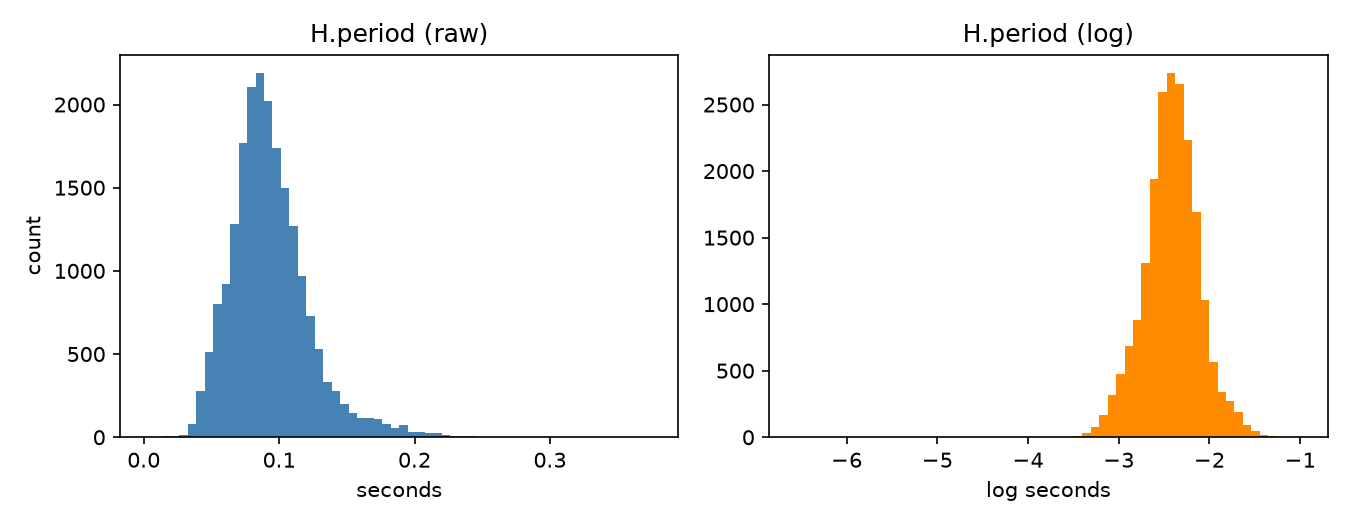
\includegraphics[width=0.85\linewidth]{hist_hold_raw_vs_log.png}
\caption{Hold time \texttt{H.period} for all subjects, raw (left) and log (right).}\label{fig:hist}
\end{figure}
\begin{figure}[H]
\centering
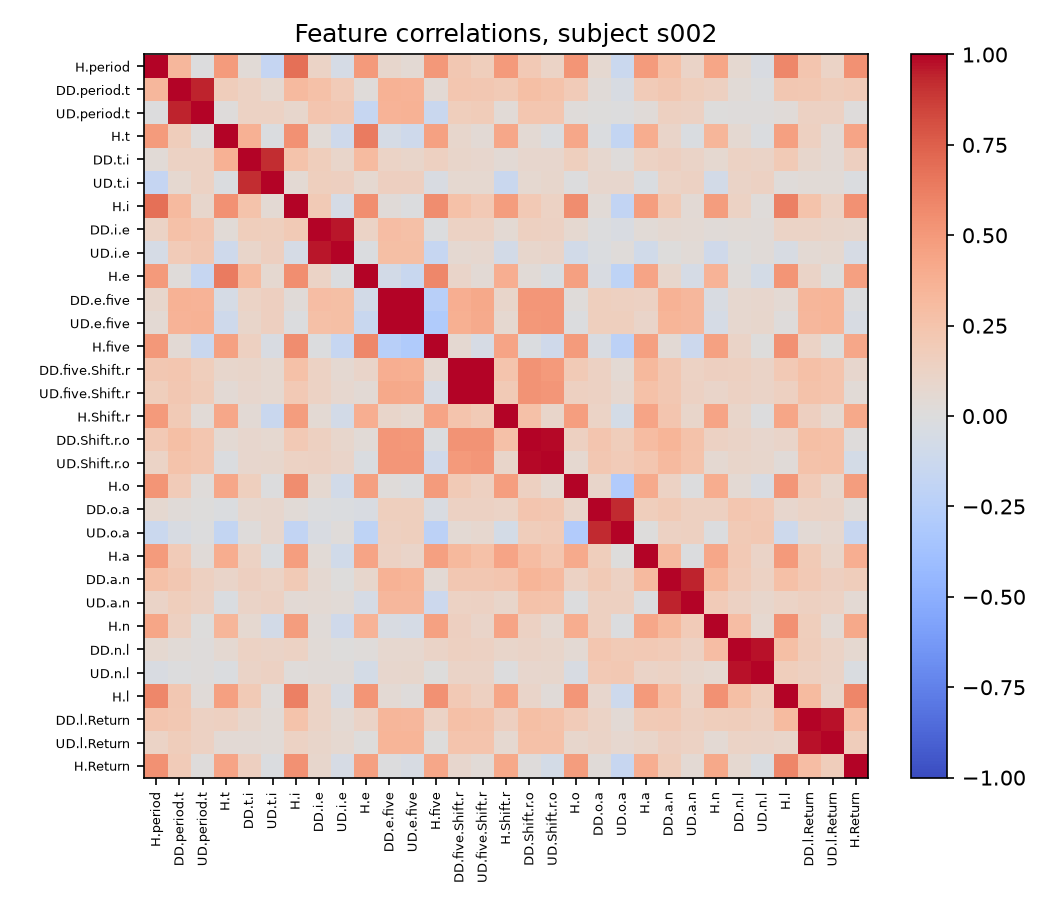
\includegraphics[width=0.7\linewidth]{corr_heatmap_user.png}
\caption{Correlations between the 31 features for subject \texttt{s002}.}
\end{figure}
\begin{figure}[H]
\centering
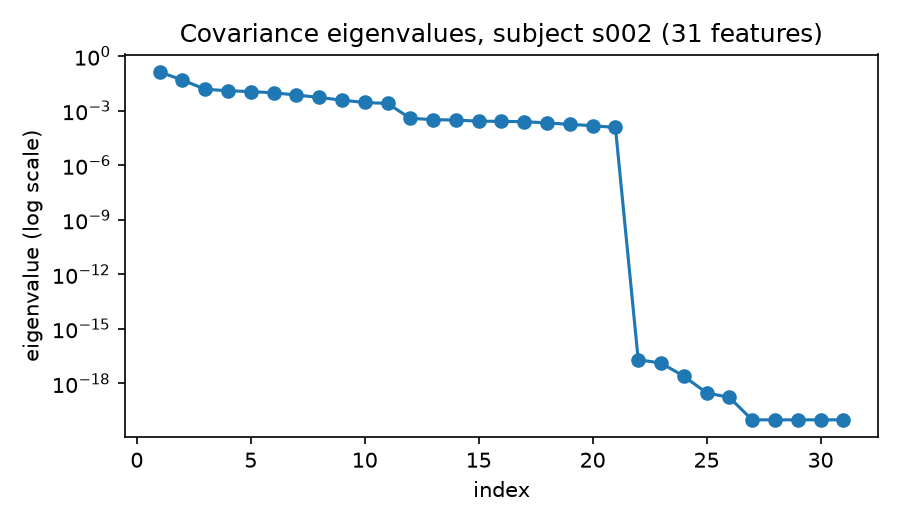
\includegraphics[width=0.6\linewidth]{eigenvalues_user.png}
\caption{Eigenvalues of the sample covariance of \texttt{s002} with all 31 features.
The last ten are numerically zero.}\label{fig:eig}
\end{figure}

\textbf{Next step (Iteration~3).} Use the 21 features H and UD, decide on the
hold-time transform, fit $\mathcal N(\hmu,\hSigma)$ on each user's early sessions,
measure false alarms on that user's later sessions and detections on the other
users, and check assumptions A1 to A6.

% =====================================================================
\section{Simulation Check}\label{sec:sim}
\subsection{Model and parameters}
All numbers come from \texttt{src/simulation.py} with seed
\texttt{np.random.default\_rng(0)}. We draw $n=5000$ points in $p=5$ dimensions from
$\mathcal N(\mu,\Sigma)$ with $\mu=0$ and $\Sigma=BB\T+5I$, where $B$ is a $5\times5$
matrix of standard normal entries. We use $\alpha=0.01$, so
$\tau=\chi^2_{5,0.99}=15.0863$, and add 50 attacks from $\mathcal N(\mu+4\cdot\one,\Sigma)$.
\[
\Sigma=\begin{pmatrix}5.74 & 1.08 & -0.93 & -0.74 & -1.07\\ 1.08 & 9.82 & -0.64 & -2.88 & -0.29\\ -0.93 & -0.64 & 12.40 & -0.22 & 0.48\\ -0.74 & -2.88 & -0.22 & 7.19 & 0.65\\ -1.07 & -0.29 & 0.48 & 0.65 & 8.27\end{pmatrix},
\qquad
\hSigma=\begin{pmatrix}5.78 & 1.20 & -0.91 & -0.92 & -1.10\\ 1.20 & 9.84 & -0.60 & -2.91 & -0.25\\ -0.91 & -0.60 & 12.21 & -0.02 & 0.67\\ -0.92 & -2.91 & -0.02 & 7.15 & 0.50\\ -1.10 & -0.25 & 0.67 & 0.50 & 8.13\end{pmatrix}.
\]
The eigenvalues of $\Sigma$ are $5.11$, $5.24$, $8.37$, $11.62$ and $13.08$, all
positive, so $\Sigma$ is PD.

\subsection{True values and estimates}
\begin{table}[H]
\centering\small
\begin{tabular}{@{}lrr@{}}
\toprule
Quantity & True & Estimate\\
\midrule
$\mu_1,\ \mu_2,\ \mu_3,\ \mu_4,\ \mu_5$ & $0,\ 0,\ 0,\ 0,\ 0$ & $0.053,\ 0.001,\ 0.023,\ 0.009,\ -0.015$\\
largest entry error $\max_{jk}|\hSigma_{jk}-\Sigma_{jk}|$ & & $0.2034$\\
relative error $\norm{\hSigma-\Sigma}_F/\norm{\Sigma}_F$ & & $0.0290$\\
mean of $d^2$ & $5$ & $5.000$\\
variance of $d^2$ & $10$ & $10.20$\\
false-alarm rate & $0.0100$ & $0.0102$\\
detection rate on the 50 attacks & $0.60$ & $0.54$\\
\bottomrule
\end{tabular}
\end{table}
The true detection rate $0.60$ is the probability that a non-central $\chi^2_5$ with
non-centrality $\delta\T\Sigma^{-1}\delta=13.0$ exceeds $\tau$ (Theorem~5(c)). With only
50 attacks its standard error is about $0.07$, so $0.54$ agrees.

\subsection{What the simulation confirms}
\begin{itemize}[nosep]
\item \textbf{Theorem 1:} $\hmu$ and $\hSigma$ are close to $\mu$ and $\Sigma$ (relative
 error $0.029$), and $\hSigma$ equals \texttt{np.cov(X, bias=True)}.
\item \textbf{Theorem 2:} all $5000$ values of $d^2$ are non-negative (the smallest is $0.060$).
\item \textbf{Theorem 3:} $d^2$ has variance $10.20$ against $2p=10$, its histogram
 follows the $\chi^2_5$ density (Figure~\ref{fig:chi2}), and a Kolmogorov-Smirnov test
 does not reject $\chi^2_5$ ($p$-value $0.47$). The mean of exactly $5$ is guaranteed by
 Corollary~\ref{cor:whitesample}.
\item \textbf{Theorem 4:} the whitened data have covariance $I$ up to $2\times10^{-15}$,
 and $W$ is symmetric with $W^2\hSigma=I$.
\item \textbf{Theorem 5:} the false-alarm rate is $0.0102$ against $\alpha=0.01$,
 within one standard error ($0.0014$).
\end{itemize}

\begin{figure}[H]
\centering
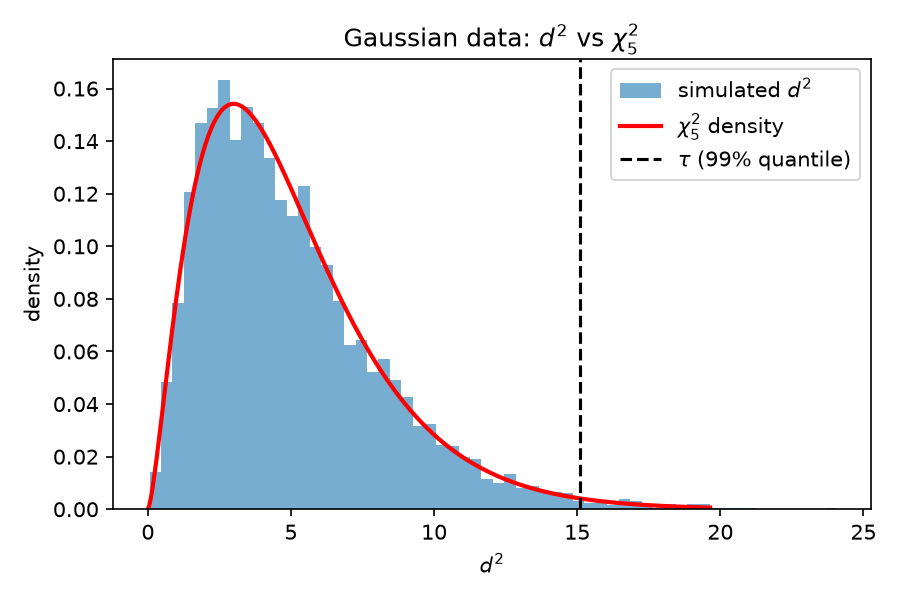
\includegraphics[width=0.62\linewidth]{sim_chi2_histogram.png}
\caption{Normal data: histogram of $d^2$ with the $\chi^2_5$ density and the threshold $\tau$.}\label{fig:chi2}
\end{figure}

\subsection{When the assumptions fail}
\textbf{Heavy tails (A2).} We redraw the data from a multivariate $t$ distribution
with 3 degrees of freedom, scaled to the same mean and covariance. Whitening still
works, because it only uses the mean and covariance, but $d^2$ no longer follows
$\chi^2_5$. The false-alarm rate is $0.057$ against $0.01$, and the Kolmogorov-Smirnov
$p$-value is numerically $0$. Over 200 repetitions the false-alarm rate is
$0.0100\pm0.0012$ for normal data and $0.0526\pm0.0042$ for $t$ data, about 5 times
too high (Figure~\ref{fig:heavy}).

\begin{figure}[H]
\centering
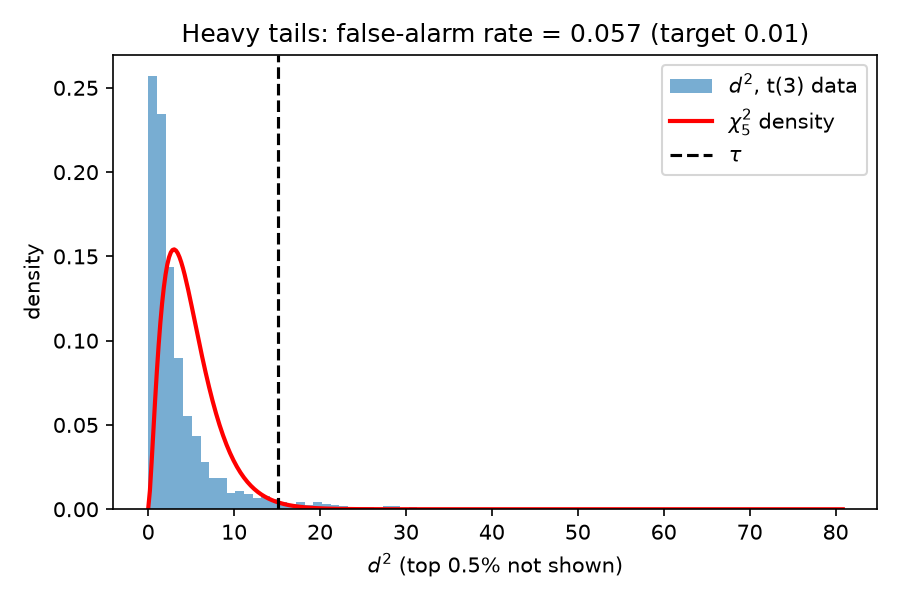
\includegraphics[width=0.62\linewidth]{sim_heavy_tail.png}
\caption{Heavy-tailed $t$ data: histogram of $d^2$ with the $\chi^2_5$ density.}\label{fig:heavy}
\end{figure}

\textbf{Small samples (A4).} We fit $\hmu,\hSigma$ on $n$ points and measure the
false-alarm rate on new points (200 repetitions for each $n$, target $0.01$). The last
column is the exact value from Theorem~5(b).

\begin{table}[H]
\centering\small
\begin{tabular}{@{}rrrr@{}}
\toprule
$n$ & relative error of $\hSigma$ & simulated false-alarm rate & Theorem~5(b)\\
\midrule
50   & 0.3156 & 0.0342 & 0.0343\\
100  & 0.2286 & 0.0183 & 0.0197\\
400  & 0.1143 & 0.0123 & 0.0120\\
1000 & 0.0712 & 0.0105 & 0.0108\\
5000 & 0.0323 & 0.0102 & 0.0102\\
\bottomrule
\end{tabular}
\end{table}
The error of $\hSigma$ falls roughly like $1/\sqrt n$, and Theorem~5(b) explains the
extra false alarms at small $n$ (Figure~\ref{fig:errn}).

\begin{figure}[H]
\centering
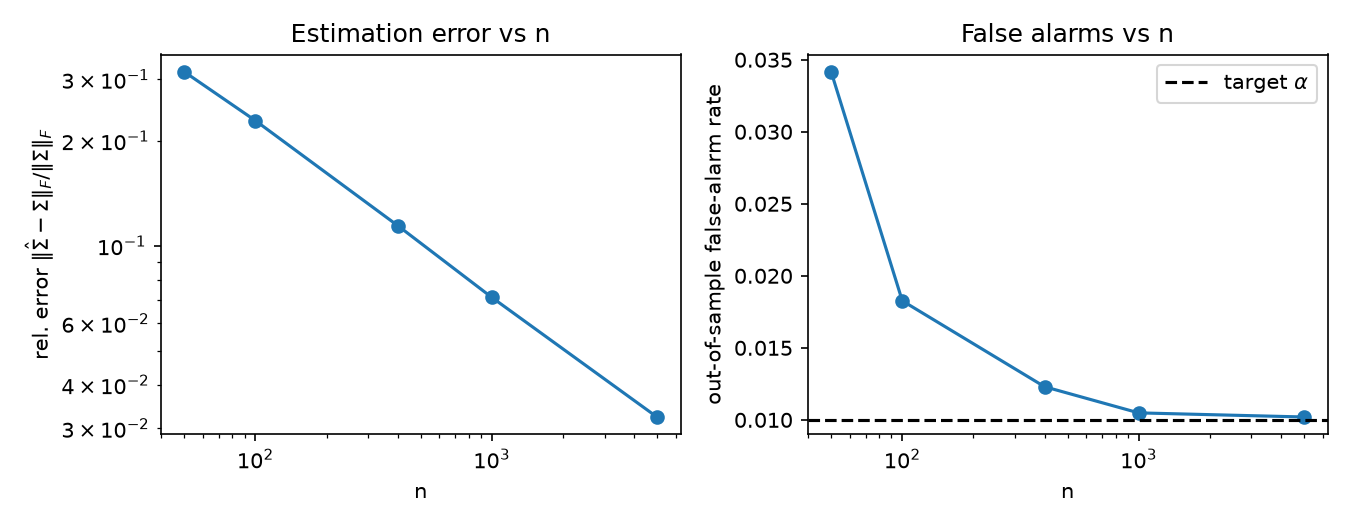
\includegraphics[width=0.9\linewidth]{sim_error_vs_n.png}
\caption{Left: relative error of $\hSigma$ against $n$ (log scales). Right: false-alarm
rate on new points against $n$, approaching the target $\alpha=0.01$.}\label{fig:errn}
\end{figure}

\textbf{Singular covariance (A3).} Adding a column equal to the sum of two others
gives a smallest eigenvalue of $1.5\times10^{-15}$, and our function
\texttt{inv\_sqrt\_psd} stops with an error. The real data behave the same way: with
all 31 features the estimate for \texttt{s002} is not PD, and with the 21 features H
and UD it is, with mean $\hat d^2=21.00=p$ as Corollary~\ref{cor:whitesample} predicts.

\textbf{First look at real data (A2).} With these 21 features, $0.150$ of
\texttt{s002}'s own attempts have $\hat d^2>\tau$, against a target of $0.01$. This is
one user, measured on the training data without a log transform, but it suggests the
real timings are not normal. We will test this properly in Iteration~3.

\bigskip
\textbf{Reference.} K.~S.~Killourhy and R.~A.~Maxion, \emph{Comparing
anomaly-detection algorithms for keystroke dynamics}, IEEE/IFIP International
Conference on Dependable Systems and Networks (DSN), 2009.

\end{document}
